\documentclass{beamer}
\usepackage[utf8]{inputenc}
\usepackage{textcomp}
\usepackage{gensymb}
\usetheme{Madrid}
\usecolortheme{default}
\usepackage{amsmath,amssymb,amsfonts,amsthm}
\usepackage{txfonts}
\usepackage{tkz-euclide}
\usepackage{listings}
\usepackage{adjustbox}
\usepackage{array}
\usepackage{tabularx}
\usepackage{gvv}
\usepackage{lmodern}
\usepackage{circuitikz}
\usepackage{tikz}
\usepackage{graphicx}

\setbeamertemplate{page number in head/foot}[totalframumber]

\usepackage{tcolorbox}
\tcbuselibrary{minted,breakable,xparse,skins}



\definecolor{bg}{gray}{0.95}
\DeclareTCBListing{mintedbox}{O{}m!O{}}{%
  breakable=true,
  listing engine=minted,
  listing only,
  minted language=#2,
  minted style=default,
  minted options={%
    linenos,
    gobble=0,
    breaklines=true,
    breakafter=,,
    fontsize=\small,
    numbersep=8pt,
    #1},
  boxsep=0pt,
  left skip=0pt,
  right skip=0pt,
  left=25pt,
  right=0pt,
  top=3pt,
  bottom=3pt,
  arc=5pt,
  leftrule=0pt,
  rightrule=0pt,
  bottomrule=2pt,
  toprule=2pt,
  colback=bg,
  colframe=orange!70,
  enhanced,
  overlay={%
    \begin{tcbclipinterior}
    \fill[orange!20!white] (frame.south west) rectangle ([xshift=20pt]frame.north west);
    \end{tcbclipinterior}},
  #3,
}
\lstset{
    language=C,
    basicstyle=\ttfamily\small,
    keywordstyle=\color{blue},
    stringstyle=\color{orange},
    commentstyle=\color{green!60!black},
    numbers=left,
    numberstyle=\tiny\color{gray},
    breaklines=true,
    showstringspaces=false,
}
%------------------------------------------------------------
%This block of code defines the information to appear in the
%Title page
\title %optional
{4.9.4}
\date{October 1,2025}
%\subtitle{A short story}

\author % (optional)
{EE25BTECH11002 - Achat Parth Kalpesh}


\begin{document}


\frame{\titlepage}

\begin{frame}{Question}

 The equations of the lines which pass through the point \brak{3, -2} and are inclined at $60\degree$ to the line $\sqrt{3} x+y=1$ is
\begin{enumerate}
\item $y+2=0$, $\sqrt{3}x-y-2-3\sqrt{3}=0$
\item $x-2=0$, $\sqrt{3}x-y+2+3\sqrt{3}=0$
\item $\sqrt{3}x-y-2-3\sqrt{3}=0$
\item None of these
\end{enumerate}
\end{frame}
\begin{frame}{Solution}
The given line can be written in normal form as
\begin{align}
    \vec{n}_1^\top \vec{x} = 1,
\end{align}
where
\begin{align}
    \vec{n}_1 = \myvec{\sqrt{3}\\1}, \quad \vec{x} = \myvec{x\\y}.
\end{align}
Let the required line have normal vector $\vec{n}=\myvec{-m\\1}$, where m is the slope of line,then its equation is
\begin{align}
    \vec{n}^\top \vec{x} = c.
\end{align}
Since the line passes through $\vec{P}=\myvec{3\\-2}$,
\begin{align}
     \vec{n}^\top \vec{P} = c
\end{align}

\end{frame}
\begin{frame}{Solution}
The angle $\theta$ between two lines is given as;
\begin{align}
    \cos\theta = \frac{\vec{n}_1^\top \vec{n}}{\norm{\vec{n}_1}\norm{\vec{n}}}.
\end{align}
Here $\theta = $60\degree$ \implies \cos\theta = \frac{1}{2}$, so
\begin{align}
    \brak{\vec{n}_1^\top \vec{n}}^2 = \frac{1}{4}\norm{\vec{n}_1}^2 \norm{\vec{n}}^2.
\end{align}
Substituting values:
\begin{align}
    \brak{-\sqrt{3}m + 1}^2 &= \frac{1}{4}\brak{4}\brak{\brak{-m}^2+1^2}\\
    \brak{-\sqrt{3}m + 1}^2 &= m^2 + 1^2\\
    3m^2 - 2\sqrt{3}m + 1 &= m^2 + 1, \\
    2m^2 &= 2\sqrt{3}m  \\
    m = 0 \text{ or } m &= \sqrt{3}
\end{align}
\end{frame}


\begin{frame}{Solution}
For m = 0 ;
\begin{align}
    \vec{n} &= \myvec{0\\1}\\
    \vec{n}^\top \vec{P} &= c
\end{align}
\begin{align}
    c = \myvec{0&1}\myvec{3\\-2}&=-2,
\end{align}
so the line is
\begin{align}
    y+2=0
\end{align}
\end{frame}


\begin{frame}{Solution}
For m = $\sqrt{3}$ ;
\begin{align}
\vec{n} &= \myvec{-\sqrt{3}\\1}\\
\vec{n}^\top \vec{P} &= c
\end{align}
\begin{align}
    c = \myvec{-\sqrt{3}&1}\myvec{3\\-2} &= -3\sqrt{3}-2
\end{align}
so the line is
\begin{align}
     \sqrt{3}x - y - 3\sqrt{3}-2 = 0
\end{align}
\end{frame}


\begin{frame}[fragile]
    \frametitle{C code}
    \begin{lstlisting}
#include <stdio.h>
#include <math.h>
void line_equation(double m, double px, double py, double *a, double *b, double *c) {
    if (isinf(m)) {
        *a = 1;
        *b = 0;
        *c = -px;
    } else {
        *a = -m;
        *b = 1;
        *c = -( (*a)*px + (*b)*py );
    }
}
    \end{lstlisting}
\end{frame}


\begin{frame}[fragile]
    \frametitle{Python Code}
    \begin{lstlisting}
import ctypes
import numpy as np
import matplotlib.pyplot as plt

lib = ctypes.CDLL(r"D:\Matgeo\4.9.4\codes\lines.so")

lib.line_equation.argtypes = [
    ctypes.c_double, ctypes.c_double, ctypes.c_double,
    ctypes.POINTER(ctypes.c_double),
    ctypes.POINTER(ctypes.c_double),
    ctypes.POINTER(ctypes.c_double)
]

# --- Python wrapper for the C function ---
def line_equation(m, px, py):
    a = ctypes.c_double()
    b = ctypes.c_double()
    c = ctypes.c_double()
    \end{lstlisting}
\end{frame}



\begin{frame}[fragile]
    \frametitle{Python Code}
    \begin{lstlisting}
    lib.line_equation(m, px, py,
                      ctypes.byref(a), ctypes.byref(b), ctypes.byref(c))
    return a.value, b.value, c.value
    # --- Given point ---
P = np.array([3, -2])

# --- Define functions for lines ---
def line_y_given_x(a, b, c, x_vals):
    # Line: ax + by + c = 0 => y = (-a*x - c)/b
    return (-a * x_vals - c) / b

# --- Given line: sqrt(3)x + y - 1 = 0 ---
a1, b1, c1 = np.sqrt(3), 1, -1

# --- Required lines ---
# Line 1: y + 2 = 0 => 0*x + 1*y + 2 = 0
a2, b2, c2 = 0, 1, 2
    \end{lstlisting}
\end{frame}


\begin{frame}[fragile]
    \frametitle{Python Code}
    \begin{lstlisting}
# Line 2: sqrt(3)x - y - (3sqrt(3)+2) = 0
a3, b3, c3 = np.sqrt(3), -1, -(3*np.sqrt(3) + 2)

# --- Generate x values over a much wider range ---
x_vals = np.linspace(-20, 25, 400)

# --- Compute y values for each line ---
y1 = line_y_given_x(a1, b1, c1, x_vals)
y2 = line_y_given_x(a2, b2, c2, x_vals)
y3 = line_y_given_x(a3, b3, c3, x_vals)
# --- Plot ---
plt.figure(figsize=(12,8))

plt.plot(x_vals, y1, 'b-', linewidth=2)
plt.plot(x_vals, y2, 'r-', linewidth=2)
plt.plot(x_vals, y3, 'g-', linewidth=2)
    \end{lstlisting}
\end{frame}


\begin{frame}[fragile]
    \frametitle{Python Code}
    \begin{lstlisting}
# Plot the common point
plt.scatter(P[0], P[1], color='k', s=80, zorder=5)
plt.text(P[0]+0.9, P[1]-2.0, "(3,-2)", fontsize=10, color='k')

# --- Place labels on the lines directly in non-overlapping positions ---
# For the blue line, place the label in the bottom-right quadrant.
# A small vertical offset (+ 0.5) is added to prevent it from sitting directly on the line.
plt.text(9, line_y_given_x(a1, b1, c1, 9) + 0.6, r'$\sqrt{3}x+y=1$', color='b', fontsize=12)

# For the red line, place the label to the right of the intersection point.
plt.text(12, line_y_given_x(a2, b2, c2, 5), r'$y+2=0$', color='r', fontsize=12)
    \end{lstlisting}
\end{frame}


\begin{frame}[fragile]
    \frametitle{Python Code}
    \begin{lstlisting}
# For the green line, place the label in the upper-right quadrant, away from the blue line's label.
plt.text(9, line_y_given_x(a3, b3, c3, 9) + 0.5, r'$\sqrt{3}x - y -(3\sqrt{3}+2)=0$', color='g', fontsize=12)

# Axes settings
plt.axhline(0, color='black', linewidth=0.7)
plt.axvline(0, color='black', linewidth=0.7)
plt.grid(True, linestyle='--', alpha=0.6)
plt.xlabel("x-axis")
plt.ylabel("y-axis")
plt.title("Lines through (3,-2) at 60° to given line")

# --- Set plot boundaries to ensure lines touch the edge ---
plt.xlim(-200, 250)
plt.ylim(-100, 100)
plt.axis("equal") 
plt.show()
    \end{lstlisting}
\end{frame}


\begin{frame}{Python Plot}
    \begin{figure}
        \centering
        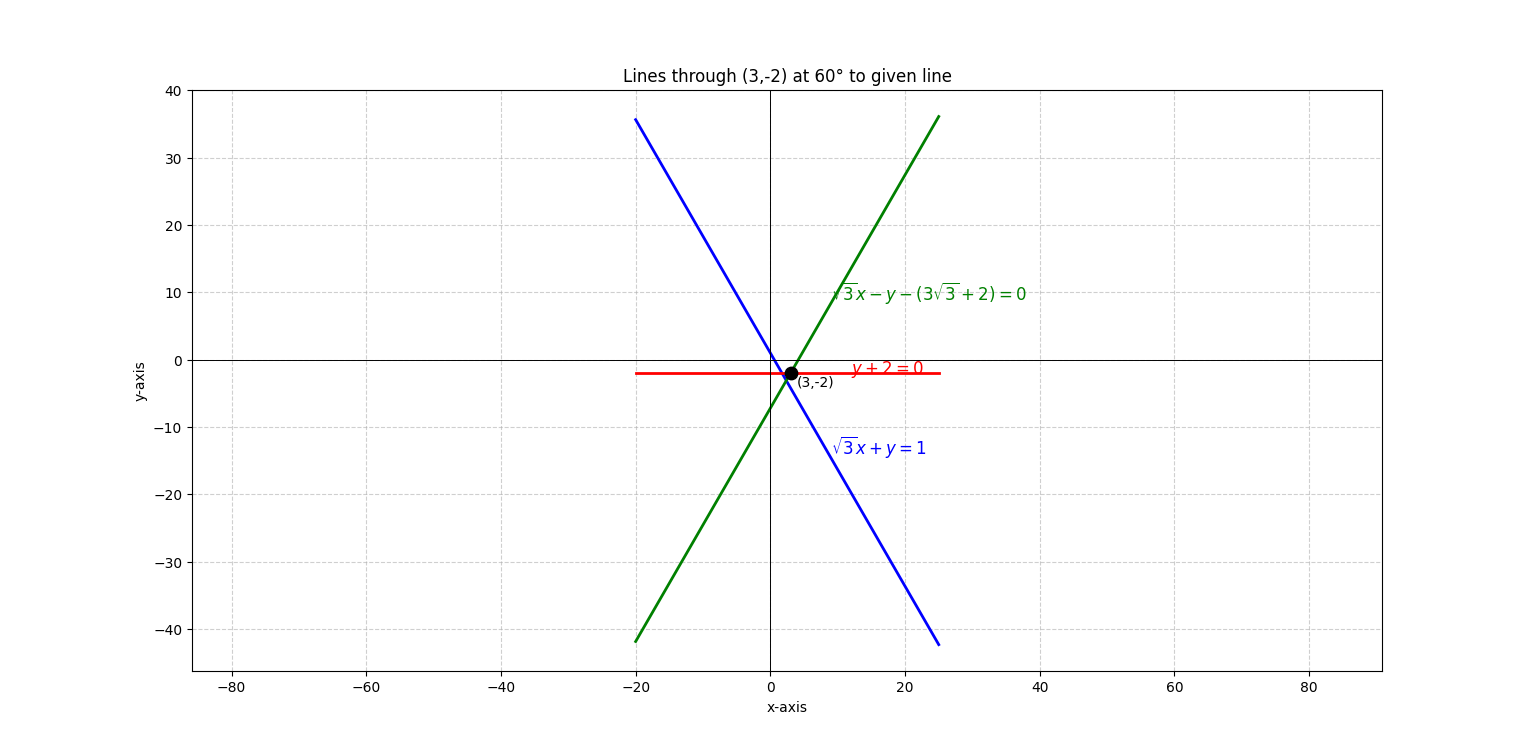
\includegraphics[width=\columnwidth]{../figs/pure_python.png}
        \caption{Lines through \brak{3,-2} at 60\degree to given line}
        \label{fig:fig}
    \end{figure}
\end{frame}
\end{document}
